\documentclass[10pt,aspectratio=169]{beamer}

\usetheme{Madrid}
\usecolortheme{seagull}
\setbeamertemplate{navigation symbols}{}
\setbeamertemplate{footline}[frame number]

\usepackage{amsmath,amssymb,bm}
\usepackage{booktabs}
\usepackage{graphicx}
\usepackage{tikz}

\title{RL Control for QEC Under Correlated Noise}
\subtitle{Steane-Code Simulation + Backend/Training Pipeline}
\author{Wenzheng Dong}
\institute{Physics Seminar}
\date{\today}

\newcommand{\improve}{\mathrm{improve(LER\sim)}}

\begin{document}

\begin{frame}
  \titlepage
\end{frame}

\begin{frame}{Motivation}
  \begin{columns}[T,onlytextwidth]
    \column{0.67\textwidth}
    \begin{itemize}
      \item Realistic hardware noise is often \textbf{temporally-correlated}, with various \textbf{types/origins} (drift, low-frequency fluctuations, crosstalk-like effects).
      \item Ignoring this can overestimate \textbf{QEC} performance under idealized i.i.d.\ assumptions.
      \item Goal: quantify how \textbf{reinforcement learning (RL)} control improves logical performance vs fixed baseline.
      \item Practical challenge: end-to-end throughput under \textbf{composed} correlated channels.
    \end{itemize}
    \column{0.33\textwidth}
    \centering
    \vspace{0.4em}
    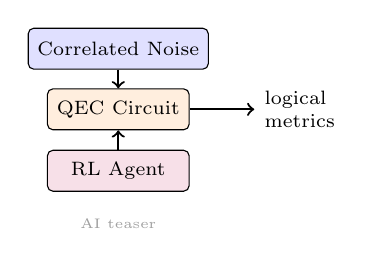
\begin{tikzpicture}[x=1cm,y=1cm,font=\scriptsize]
      \node[draw,rounded corners=2pt,fill=blue!12,minimum width=1.8cm,minimum height=0.52cm] (n) at (0,1.35) {Correlated Noise};
      \node[draw,rounded corners=2pt,fill=orange!13,minimum width=1.8cm,minimum height=0.52cm] (q) at (0,0.58) {QEC Circuit};
      \node[draw,rounded corners=2pt,fill=purple!12,minimum width=1.8cm,minimum height=0.52cm] (r) at (0,-0.20) {RL Agent};
      \draw[->,thick] (n) -- (q);
      \draw[->,thick] (r) -- (q);
      \draw[->,thick] (q.east) -- +(0.82,0) node[right,align=left] {\scriptsize logical\\\scriptsize metrics};
      \node[align=center,font=\tiny,text=gray!75] at (0,-0.88) {AI teaser};
    \end{tikzpicture}
  \end{columns}
\end{frame}

\begin{frame}{System Picture}
  \begin{center}
    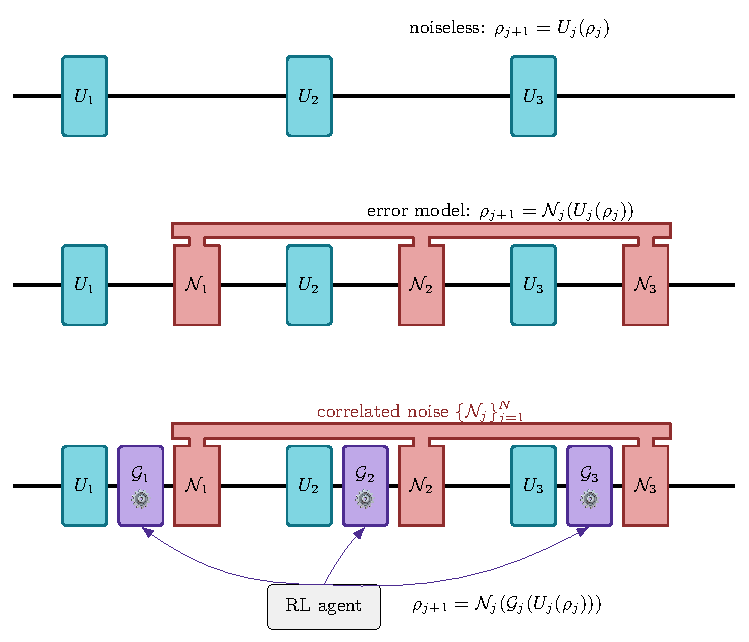
\includegraphics[height=0.58\textheight,keepaspectratio]{rl_qec_channel_abstract_tikz.pdf}
  \end{center}
  \small
  Noisy controlled evolution:
  \[
    \rho_{j+1}
    =
    \mathcal{N}^{\mathrm{corr}}_j
    \!\Big(
    \mathcal{G}^{(u_j)}_j
    \!\big(U_j\rho_j U_j^\dagger\big)\Big).
  \]
\end{frame}

\begin{frame}{Physical Meaning of \texorpdfstring{$\mathcal{G}$}{G} and \texorpdfstring{$\mathcal{N}$}{N}}
  \small
  \begin{itemize}
    \item \textbf{Yes}: gate-depolarization is used as an effective model of \textbf{gate-operation-associated} noise.
    \item \textbf{Yes}: correlated channel is used as \textbf{environment/background} noise with temporal memory.
    \item \(\mathcal{G}^{(u_j)}_j\) acts on gate controls (1q/2q slots); in the composed model, \(\mathcal{N}^{\mathrm{corr}}_j\) strength can couple to control mismatch, while correlation structure (\(f,\gamma\)) remains environmental.
  \end{itemize}
  \vspace{0.3em}
  \[
    \rho_{j+1}
    =
    \mathcal{N}^{\mathrm{corr}}_j
    \!\Big(
    \mathcal{G}^{(u_j)}_j
    \!\big(U_j\rho_j U_j^\dagger\big)\Big).
  \]
  \small
  Here \(u_j\) is produced by RL policy; \(\mathcal{N}^{\mathrm{corr}}_j\) mainly acts during idle windows.
\end{frame}

\begin{frame}{Physical Picture of Two Noise Layers}
  \centering
  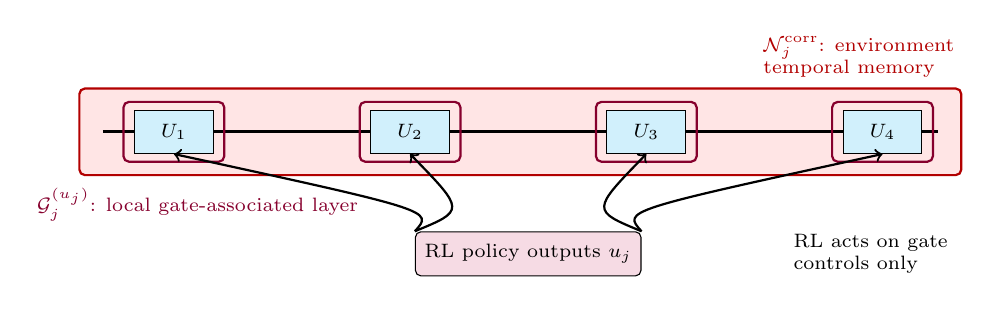
\begin{tikzpicture}[x=1cm,y=1cm,font=\scriptsize]
    % Correlated environmental layer across time.
    \fill[red!10,rounded corners=2pt] (0.3,-0.55) rectangle (11.5,0.55);
    \draw[red!70!black,thick,rounded corners=2pt] (0.3,-0.55) rectangle (11.5,0.55);
    \node[red!70!black,align=left] at (10.2,0.95) {\(\mathcal{N}^{\mathrm{corr}}_j\): environment\\temporal memory};

    % Circuit timeline.
    \draw[very thick] (0.6,0) -- (11.2,0);
    \node[draw,fill=cyan!18,minimum width=1.00cm,minimum height=0.55cm] (u1) at (1.5,0) {\(U_1\)};
    \node[draw,fill=cyan!18,minimum width=1.00cm,minimum height=0.55cm] (u2) at (4.5,0) {\(U_2\)};
    \node[draw,fill=cyan!18,minimum width=1.00cm,minimum height=0.55cm] (u3) at (7.5,0) {\(U_3\)};
    \node[draw,fill=cyan!18,minimum width=1.00cm,minimum height=0.55cm] (u4) at (10.5,0) {\(U_4\)};

    % Gate-associated noise wrappers.
    \node[draw=purple!70!black,thick,rounded corners=2pt,minimum width=1.28cm,minimum height=0.76cm] at (u1) {};
    \node[draw=purple!70!black,thick,rounded corners=2pt,minimum width=1.28cm,minimum height=0.76cm] at (u2) {};
    \node[draw=purple!70!black,thick,rounded corners=2pt,minimum width=1.28cm,minimum height=0.76cm] at (u3) {};
    \node[draw=purple!70!black,thick,rounded corners=2pt,minimum width=1.28cm,minimum height=0.76cm] at (u4) {};
    \node[purple!70!black,align=left] at (1.8,-0.92) {\(\mathcal{G}^{(u_j)}_j\): local gate-associated layer};

    % RL control connections.
    \node[draw,rounded corners=2pt,fill=purple!14,minimum width=2.15cm,minimum height=0.56cm] (rl) at (6.0,-1.55) {RL policy outputs \(u_j\)};
    \draw[->,thick] (rl.north west) .. controls (4.8,-1.0) .. (u1.south);
    \draw[->,thick] (rl.north west) .. controls (5.2,-1.0) .. (u2.south);
    \draw[->,thick] (rl.north east) .. controls (6.8,-1.0) .. (u3.south);
    \draw[->,thick] (rl.north east) .. controls (7.2,-1.0) .. (u4.south);
    \node[align=left] at (10.35,-1.55) {RL acts on gate\\controls only};
  \end{tikzpicture}

  \vspace{0.35em}
  \small
  \[
    \rho_{j+1}
    =
    \mathcal{N}^{\mathrm{corr}}_j
    \!\Big(
    \mathcal{G}^{(u_j)}_j
    \!\big(U_j\rho_j U_j^\dagger\big)\Big).
  \]
\end{frame}

\begin{frame}{Google-Style Noise Coverage: What We Do Not Yet Model}
  \small
  \begin{columns}[T,onlytextwidth]
    \column{0.50\textwidth}
    \textbf{Reported in Google paper / supplement}
    \begin{itemize}
      \item Pauli characterization includes 1q, 2q, measurement, and DD-during-readout/reset error components.
      \item Drift scenarios include step-like, sinusoidal, and stroboscopic profiles over CZ coupling, XY amplitude, and frequency.
      \item Control space includes pulse-level knobs: DRAG terms, CZ detunings, transfer-function settling/reflection, virtual-\(Z\) phase corrections.
    \end{itemize}
    \column{0.50\textwidth}
    \textbf{Not yet explicit in our current simulator}
    \begin{itemize}
      \item No explicit measurement/readout/reset error channel (we focus on gate depolarization + correlated idle Pauli).
      \item No explicit pulse-transfer-function distortion model.
      \item No explicit context-dependent coherent phase/crosstalk error model.
      \item Control-to-noise map is low-dimensional effective mapping, not full pulse-parameter space per gate.
    \end{itemize}
  \end{columns}
  \vspace{0.25em}
  \tiny
  Source anchors: Google paper Fig. 4 text; Supplement Sec. I.A, II.A, V.A/B.
\end{frame}

\begin{frame}{Important Noise Directions Beyond Both Studies}
  \small
  \begin{itemize}
    \item \textbf{Leakage dynamics}: explicit \(|2\rangle\)-state population flow across cycles, including leakage propagation and repumping.
    \item \textbf{Non-Pauli coherent accumulation}: systematic over/under-rotation, spectator-\(ZZ\), and coherent phase buildup not reduced to depolarizing/Pauli.
    \item \textbf{Burst/heavy-tail events}: rare but high-impact events (e.g., quasiparticle bursts / cosmic-ray-like faults) causing multi-qubit transients.
    \item \textbf{Multi-timescale nonstationarity}: \(1/f\) + random-walk + abrupt jumps, beyond simple sinusoidal drift or two-state Markov telegraph.
    \item \textbf{Long-range spatial correlation}: chip-wide or bus-mediated correlated faults (including correlated readout excursions).
  \end{itemize}
  \vspace{0.25em}
  \small
  These directions likely require a richer simulator architecture (hybrid hidden-state noise, pulse-level abstractions, and co-training with decoder adaptation).
\end{frame}

\begin{frame}{Minimal Physics Model Used in Simulation}
  \small
  \textbf{Control-to-gate-noise map} (for gate event \(e\), slot \(s(e)\)):
  \[
    p_{1q}^{(e)}=\mathrm{clip}\!\left(p_{1q}^{\mathrm{base}}+\alpha_{1q}\big(u_{1q,s(e)}-u_{1q,s(e)}^\star(t)\big)^2,\,0,\,p_{\max}\right),
  \]
  \[
    p_{2q}^{(e)}=\mathrm{clip}\!\left(p_{2q}^{\mathrm{base}}+\alpha_{2q}\big(u_{2q,s(e)}-u_{2q,s(e)}^\star(t)\big)^2,\,0,\,p_{\max}\right).
  \]

  \vspace{0.25em}
  \textbf{Correlated environmental channel} (two-state Markov telegraph):
  \[
    \gamma=\frac{1-e^{-f\Delta t}}{2},\quad
    T=
    \begin{bmatrix}
      1-\gamma & \gamma\\
      \gamma & 1-\gamma
    \end{bmatrix},
    \quad \Delta t=200\,\mathrm{ns}.
  \]
  \[
    p_{\mathrm{target}}=\mathrm{clip}\!\left(\big(p_{1q}^{\mathrm{base}}+\alpha_{1q}\overline{(u-u^\star)^2}\big)g,0,p_{\max}\right),
    \quad
    p_{\mathrm{idle}}=1-(1-p_{\mathrm{target}})^{1/N_w}.
  \]
\end{frame}

\begin{frame}{Experimental Setup (Physics View)}
  \begin{itemize}
    \item Platform-level model: Steane memory experiment with repeated stabilizer rounds.
    \item Noise decomposition: gate-associated effective depolarization + temporally correlated environmental idle noise.
    \item Control objective: RL learns gate controls to improve logical metrics under non-i.i.d.\ noise.
    \item Main comparison: learned policy vs fixed-zero policy over many seeds.
  \end{itemize}
\end{frame}

\begin{frame}{What We Optimized Practically}
  \begin{itemize}
    \item Simulator kernels for correlated/composed channels (to make large-seed studies feasible).
    \item RL-side training/evaluation throughput for stable statistical conclusions.
    \item Staged benchmark design over \((f,g)\), then confirm runs with increasing seed count.
  \end{itemize}
\end{frame}

\begin{frame}{Backend Speedup (Kernel-Dominated A/B)}
  \begin{table}
    \centering
    \small
    \begin{tabular}{lccc}
      \toprule
      Channel & old (s) & new (s) & speedup \\
      \midrule
      \texttt{google\_gate\_specific} & 0.284 & 0.311 & 0.91x \\
      \texttt{correlated\_pauli\_noise\_channel} & 4.759 & 0.437 & 10.89x \\
      \texttt{composed\_google\_gate\_specific\_correlated} & 10.670 & 0.597 & 17.87x \\
      \bottomrule
    \end{tabular}
  \end{table}
  \small
  For target correlated/composed channels, simulator-side acceleration is substantial.
\end{frame}

\begin{frame}{Benchmark Plan for RL Advantage}
  \begin{itemize}
    \item Grid and focus over correlated parameters:
    \[
      f \in \{10^2,10^3,10^4\},\quad g \in \{0.4,1.0,1.6\}.
    \]
    \item Multi-phase design:
    \begin{itemize}
      \item quick grid $\rightarrow$ pilot focus $\rightarrow$ confirm (10 seeds) $\rightarrow$ confirm (40 seeds).
    \end{itemize}
    \item Key condition selected by stability and effect size:
    \[
      f=10^4,\ g=0.4.
    \]
  \end{itemize}
\end{frame}

\begin{frame}{Fig.13: Phase1 Grid (What This Figure Means)}
  \scriptsize
  \textbf{Definitions:}
  \begin{itemize}
    \item \textbf{Phase1} = quick screen on 9 \((f,g)\) points (3 frequencies \(\times\) 3 strengths).
    \item \(\Delta\)\textbf{success} \(=\) \texttt{success\_rate(learned)} \(-\) \texttt{success\_rate(fixed\_zero)}.
    \item \textbf{learned-fixed (pp)} means this difference in \textbf{percentage points} (pp).
  \end{itemize}
  \vspace{-0.1em}
  \begin{center}
    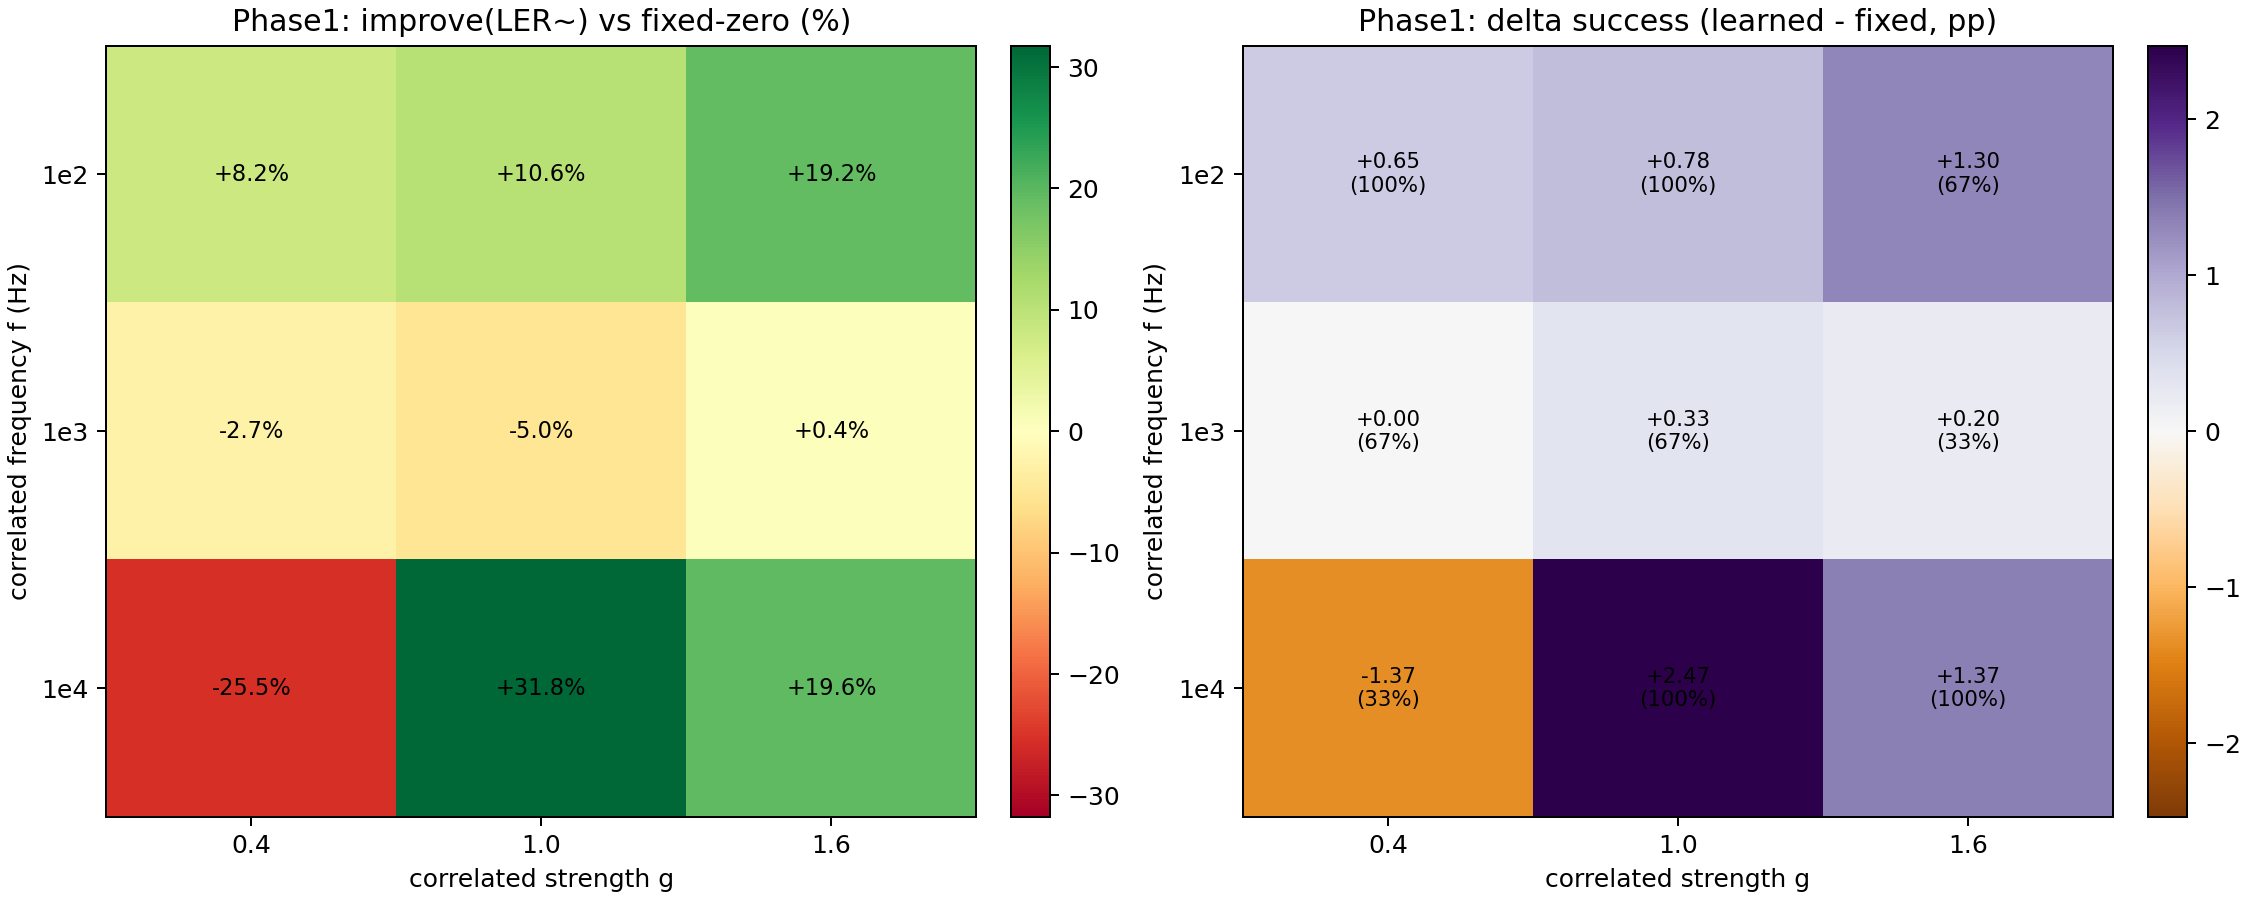
\includegraphics[width=0.76\linewidth]{../../code/data_generated/benchmarks/composed_corr_fg/plots_20260309/phase1_heatmaps_rl_advantage.png}
  \end{center}
  This is a screening map to select conditions for deeper confirm runs.
\end{frame}

\begin{frame}{Fig.14: Top-Condition Ablation (What Is Being Compared)}
  \scriptsize
  \textbf{Ablation} = controlled comparison where only one design choice changes at a time
  (same top condition \(f=10^4, g=0.4\), same benchmark protocol).
  \begin{itemize}
    \item \textbf{Fast eval}: no shot traces; uses summary/proxy metrics; much faster.
    \item \textbf{Trace eval}: stores shot traces and detector histories; higher fidelity, slower.
  \end{itemize}
  \begin{center}
    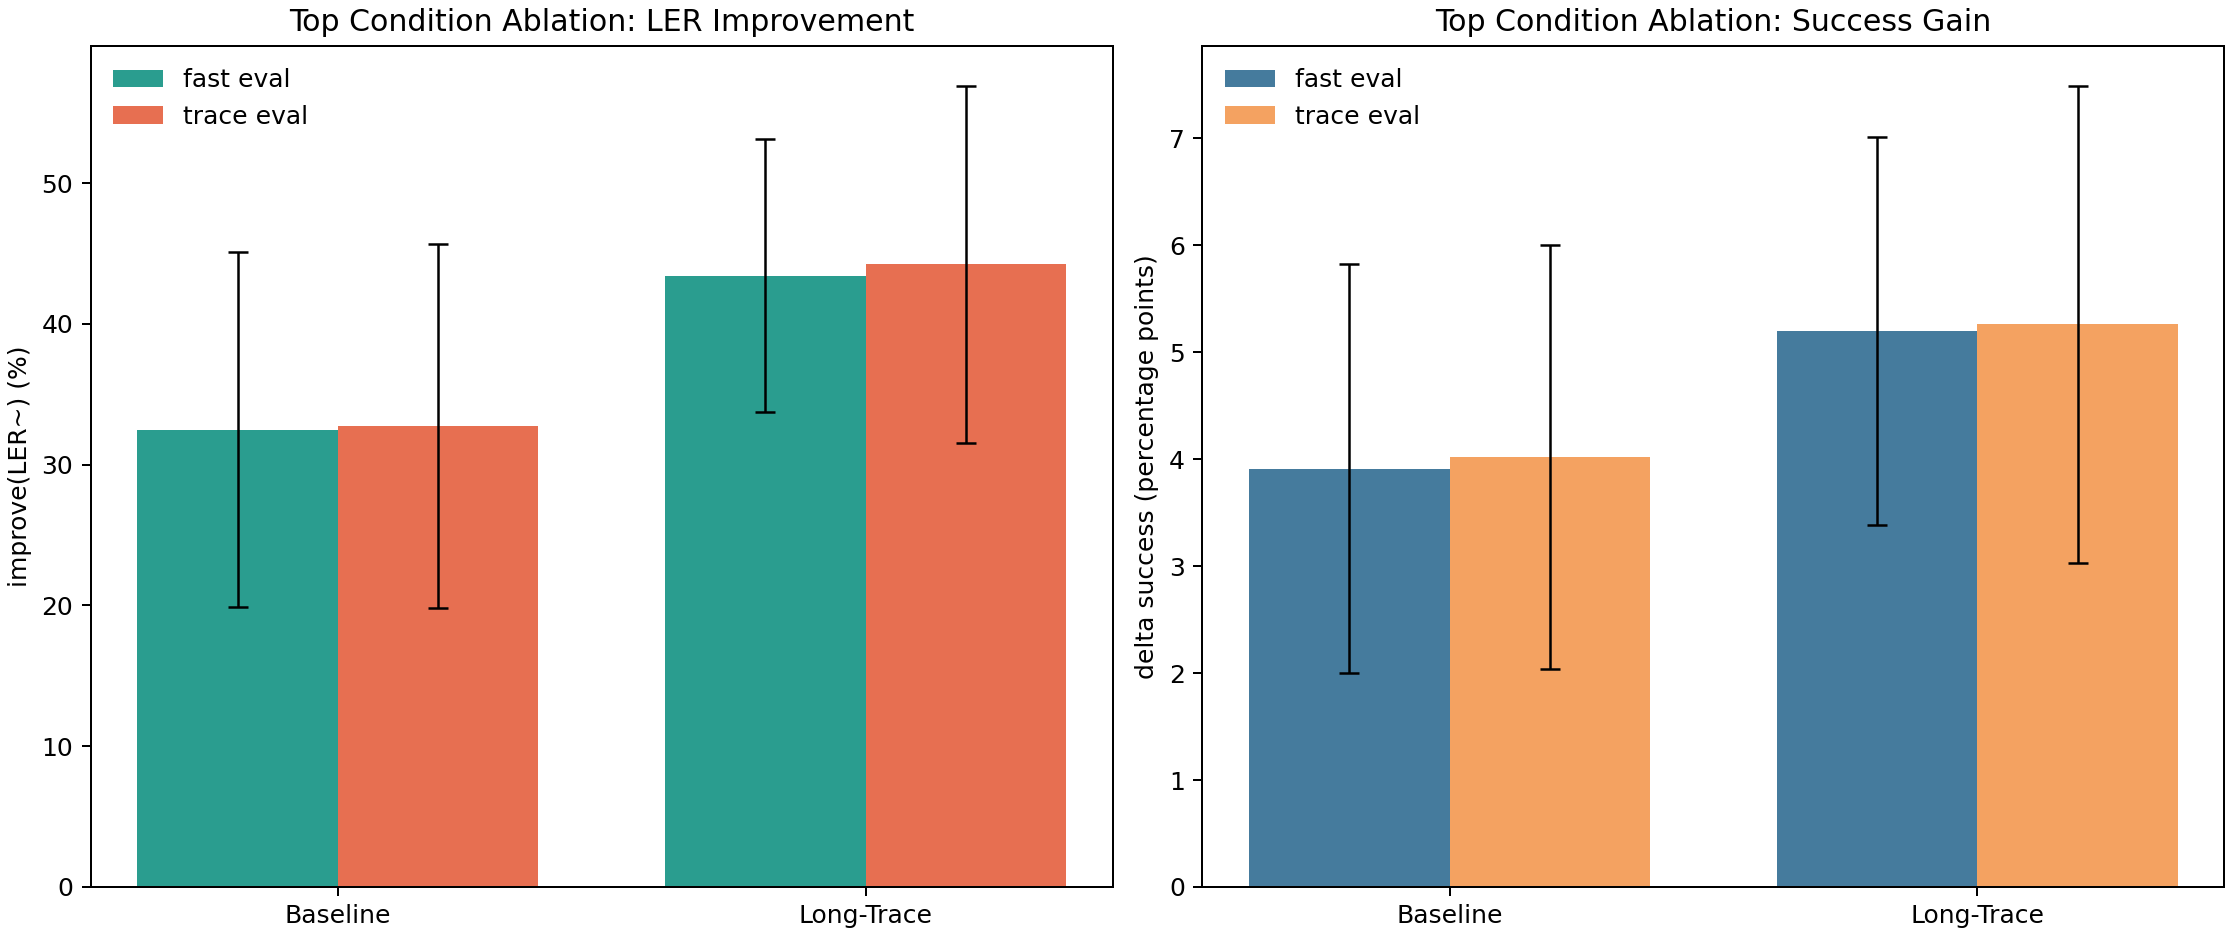
\includegraphics[width=0.84\linewidth]{../../code/data_generated/benchmarks/composed_corr_fg/phase6_20260310_confirm40/topcond_ablation_fast_vs_trace.png}
  \end{center}
  Error bars here are \texttt{std} (not 95\% CI).
\end{frame}

\begin{frame}{Fig.15: Confirm10 vs Confirm40 (Why Two Confirms)}
  \small
  \begin{itemize}
    \item \textbf{Confirm10} = same condition and model, averaged over 10 random seeds.
    \item \textbf{Confirm40} = same thing, but 40 seeds for tighter uncertainty.
    \item Purpose: not to change method, only to improve statistical confidence.
  \end{itemize}
  \begin{center}
    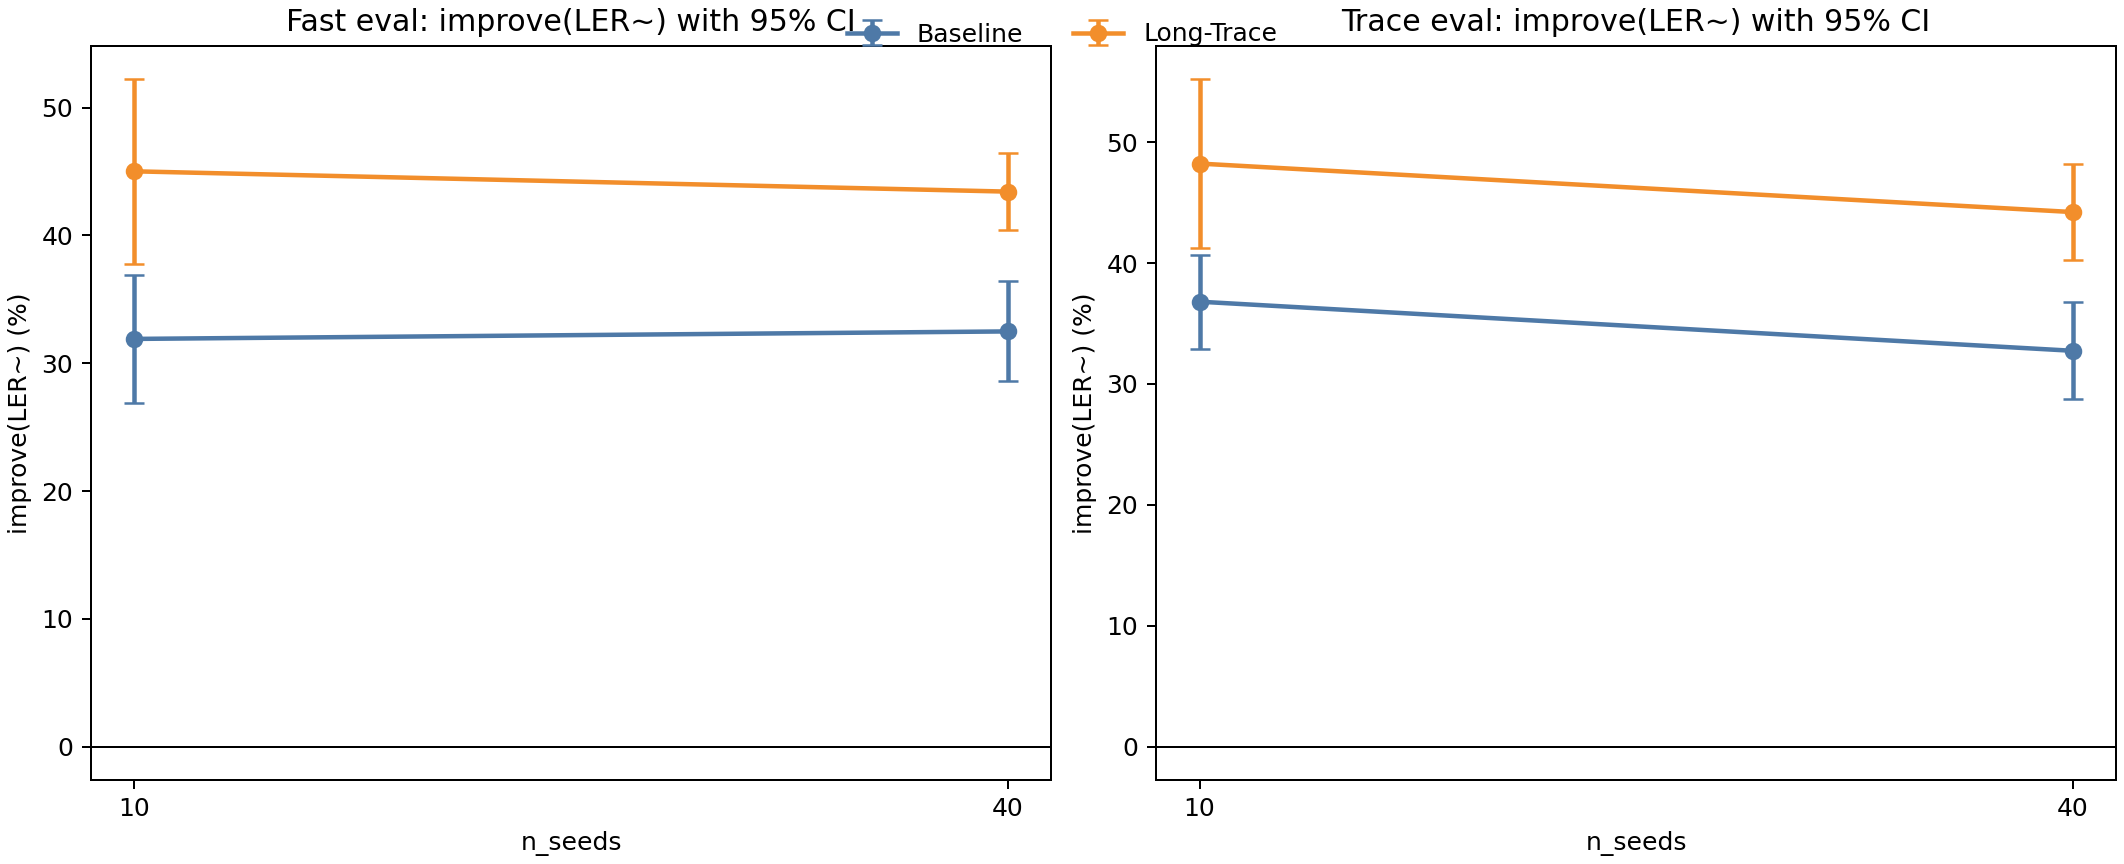
\includegraphics[width=0.84\linewidth]{../../code/data_generated/benchmarks/composed_corr_fg/plots_20260310/topcond_confirm10_vs_40_ci95.png}
  \end{center}
  \small
  CI half-width formula: $\mathrm{CI95}_{1/2}=1.96\cdot \mathrm{std}/\sqrt{n_{\text{seeds}}}$.
\end{frame}

\begin{frame}{Numerical Result at $f=10^4,\ g=0.4$}
  \small
  Metric shown: $\improve$ (mean $\pm$ CI95 half-width)
  \vspace{0.4em}
  \begin{table}
    \centering
    \begin{tabular}{lcc}
      \toprule
      Run & Fast eval & Trace eval \\
      \midrule
      confirm10 baseline & 31.90\% $\pm$ 5.02\% & 36.81\% $\pm$ 3.88\% \\
      confirm10 long-trace & 45.01\% $\pm$ 7.23\% & 48.23\% $\pm$ 7.01\% \\
      confirm40 baseline & 32.49\% $\pm$ 3.91\% & 32.74\% $\pm$ 4.00\% \\
      confirm40 long-trace & 43.43\% $\pm$ 3.01\% & 44.22\% $\pm$ 3.94\% \\
      \bottomrule
    \end{tabular}
  \end{table}
\end{frame}

\begin{frame}{Takeaways}
  \begin{itemize}
    \item \textbf{RL advantage} is \textbf{positive} and \textbf{reproducible} under composed correlated noise.
    \item Increasing \textbf{seeds} (10 $\rightarrow$ 40) narrows \textbf{uncertainty}; effect becomes more statistically stable.
    \item \textbf{Long-trace} variant consistently outperforms \textbf{baseline} on the top condition.
    \item \textbf{Backend optimization} is necessary but not sufficient; \textbf{training/eval protocol} matters.
  \end{itemize}
\end{frame}

\begin{frame}{Next Steps}
  \begin{itemize}
    \item \textbf{Incorporate measurement errors}: add stabilizer readout channel (start with symmetric flip, then asymmetric/correlated variants).
    \item Extend controlled scans over broader $(f,g)$ regimes with fixed evaluation protocol.
    \item Test transferability to additional correlated/noise families.
    \item Strengthen claims with pre-registered statistical criteria and standardized CI reporting.
  \end{itemize}
\end{frame}

\begin{frame}
  \centering
  \Large Thank you.
\end{frame}

\end{document}
